\clearpage
\subsection{User Interface \& System Visualization}
To bridge the gap between the complex cognitive backend and the end-user, a dedicated web application was developed. The frontend is built using React an d Vite, utilizing Tailwind CSS for responsive and modern styling. The project follows a modular architecture, dividing the interface into reusable \texttt{components}, dedicated \texttt{pages}, and API \texttt{services} for seamless backend integration. The application features a side navigation menu providing access to four primary functional modules.

\subsubsection{Authentication Gateway (Login Page)}
\begin{figure}[H]
\centering
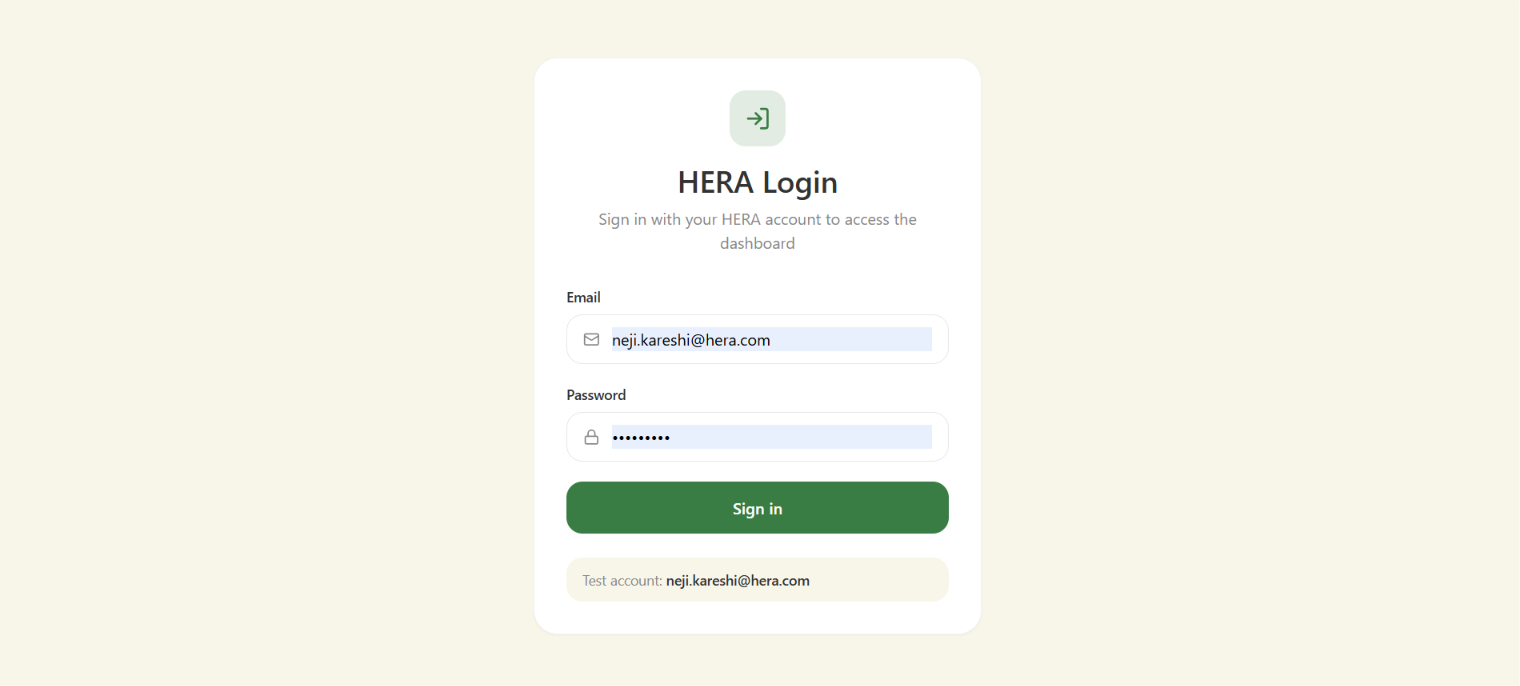
\includegraphics[width=0.8\textwidth]{image/UI/login.png}
\caption{Login Interface}
\label{fig:LOGIN}
\end{figure}

The \textbf{Login Page} serves as the secure entry point to the H.E.R.A. ecosystem, ensuring that situational data and home controls are accessible only to authorized residents. Following the system's core design philosophy, the interface utilizes a centered authentication card with soft rounded corners, set against a calming off-white background. \\

The interface features minimalist credential fields within a clean, flat design, utilizing sage green accents to maintain visual consistency with the main dashboard. Overall, this distraction-free layout ensures a focused, frictionless, and secure authentication process.



\subsubsection{Home (Unified Control Center)}

\begin{figure}[H]
    \centering
	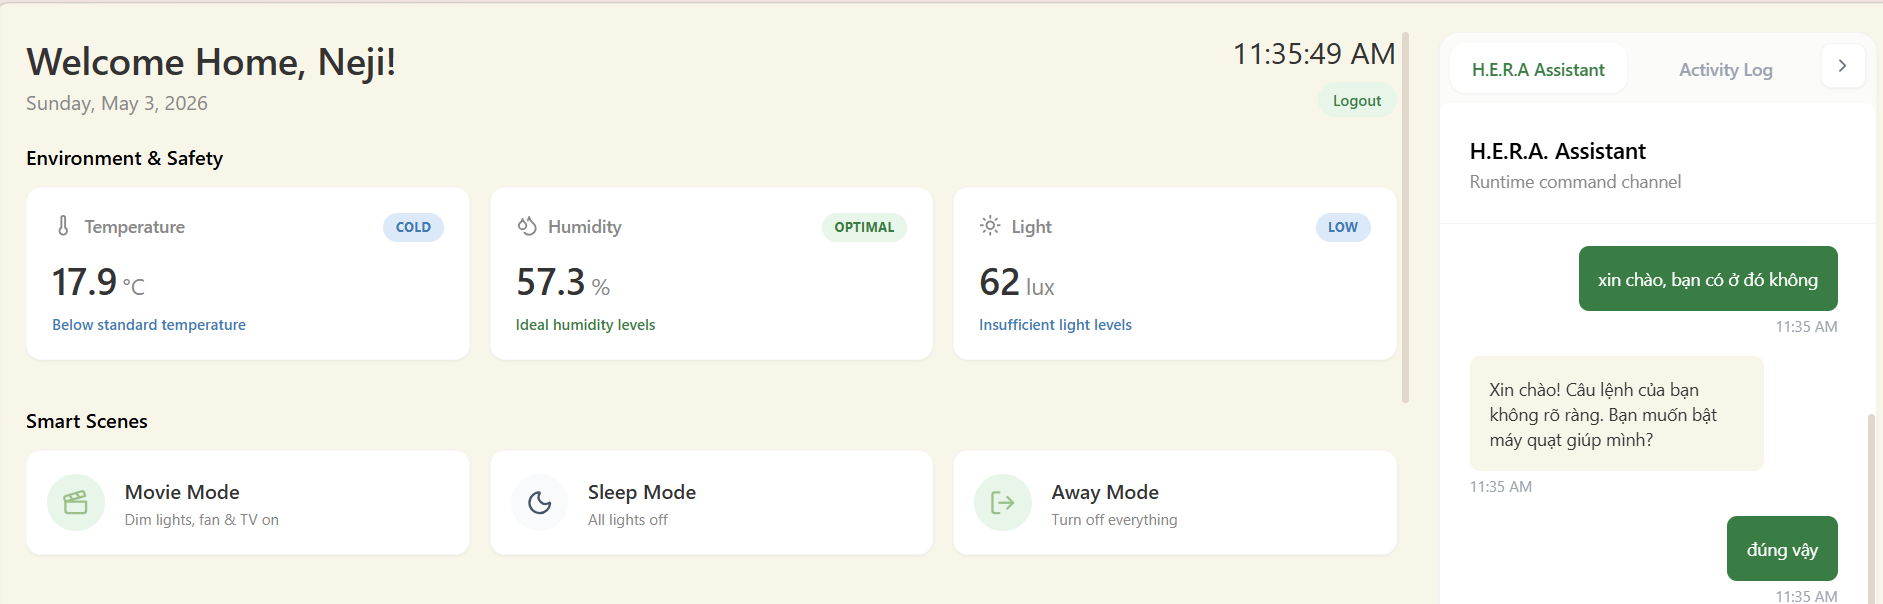
\includegraphics[width=0.95\textwidth]{image/UI/home.png}
    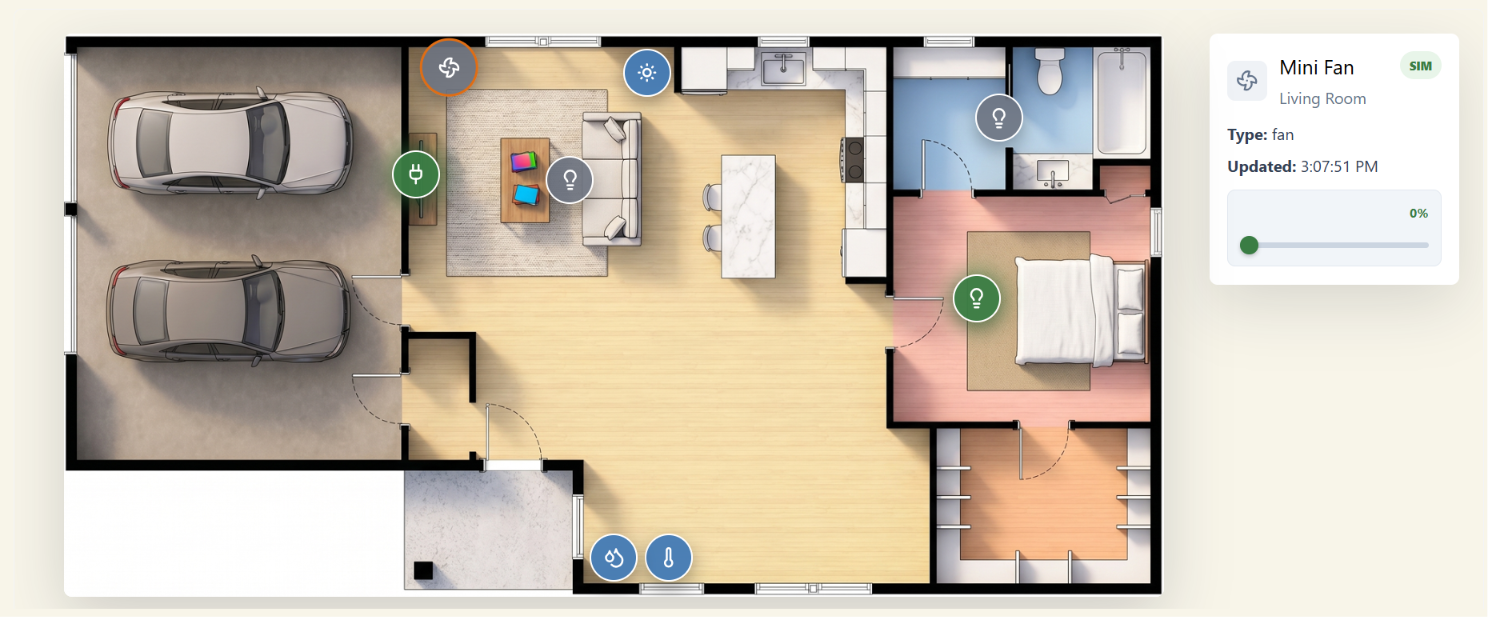
\includegraphics[width=0.95\textwidth]{image/UI/house.png}
    \caption{H.E.R.A. Home Dashboard featuring the Interactive Floor Plan, Smart Scenes, and Multilingual AI Assistant.}
    \label{fig:home_page_new}
\end{figure}

The Home page serves as the primary operational hub, offering comprehensive situational awareness and intuitive control mechanisms. Designed with a clean, minimalist, and warm aesthetic utilizing soft cream, beige, and pastel tones, the interface minimizes cognitive load while integrating four main functional areas:

\begin{itemize}
    \item \textbf{Environment \& Safety Context:} Displays real-time telemetry such as Temperature, Humidity, and Light intensity. Going beyond raw numerical data, this module provides instant contextual evaluation via color-coded badges (e.g., "COLD", "OPTIMAL", "LOW") and descriptive subtexts (e.g., "Below standard temperature", "Insufficient light levels"), allowing residents to quickly assess the comfort level of their home.

    \item \textbf{Smart Scenes:} A newly introduced module offering macro-level automation presets. Users can trigger predefined operational modes with a single click. Current presets include "Movie Mode" (dims lights, activates fan and TV), "Sleep Mode" (deactivates all lighting), and "Away Mode" (powers down all non-essential appliances for energy conservation and security).

    \item \textbf{Interactive House Floor Plan \& Integrated Controls:} A spatial visualization feature that maps the physical layout of the residence (including garage, living room, bedroom, and bathroom). IoT devices and sensors are represented as interactive nodes mapped to their exact physical locations. This module streamlines device management by integrating direct controls directly into the map: a \textbf{left-click} on a node acts as a quick toggle to instantly turn the appliance on or off, while a \textbf{right-click} opens a detailed contextual menu. This menu displays the device type, current state, data source, last updated timestamp, and supports continuous control inputs (e.g., adjusting the living room fan speed dynamically via a slider).

    \item \textbf{H.E.R.A. Assistant \& Activity Log:} Positioned on the right sidebar, this module features a built-in chat interface connecting directly to the multi-agent AI pipeline. It seamlessly handles natural language requests and supports multilingual interactions (e.g., processing Vietnamese inputs such as \textit{"xin chào, bạn có ở đó không"}). It accommodates both text input and dedicated Voice Commands. Furthermore, an "Activity Log" tab is integrated to maintain an accessible audit trail of system events and command histories.
\end{itemize}

\subsubsection{Analytics (Environmental Trends)}
% Chèn hình ảnh giao diện Analytics vào đây
\begin{figure}[H]
	\centering
	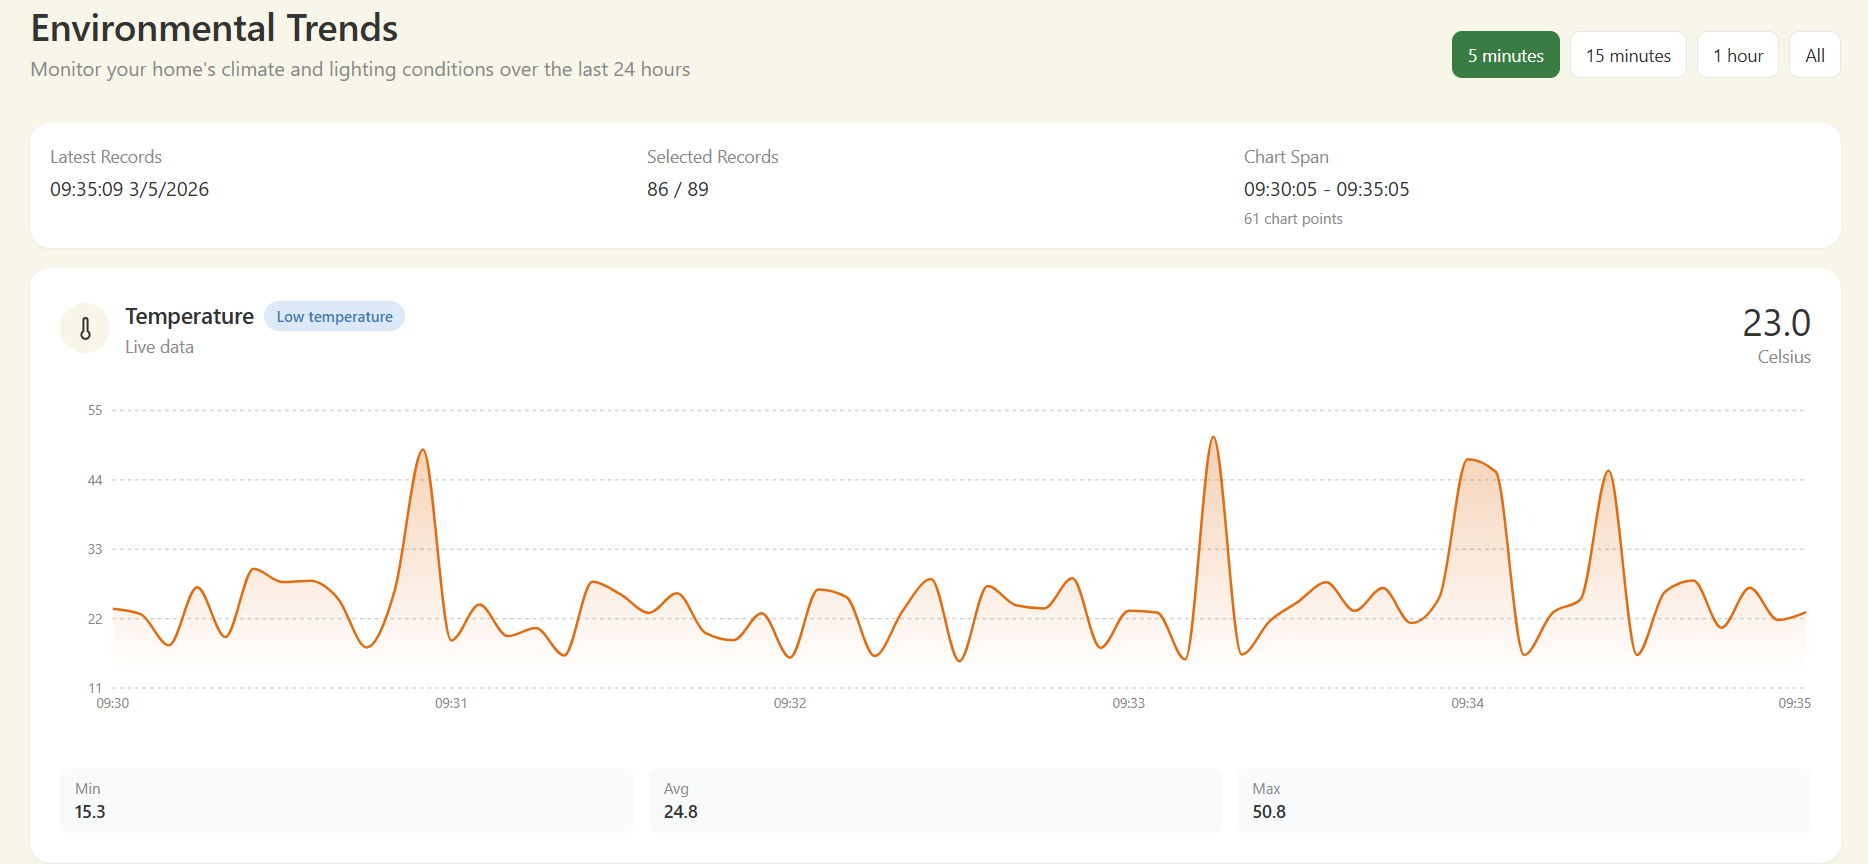
\includegraphics[width=0.95\textwidth]{image/UI/analytic.png}
	\caption{Analytic Page}
	\label{fig:ANALYTIC}
\end{figure}
To support the system's proactive energy management and monitoring goals, the Analytics module visualizes time-series data. It renders continuous line charts for telemetry streams (such as Temperature and Relative Humidity), displaying live data points alongside aggregated metrics (Minimum, Average, Maximum). This empowers users to monitor historical patterns and visually verify the operational effectiveness of the predictive models.